\documentclass{standalone}
\usepackage{tikz}
\usetikzlibrary{patterns, positioning}


\begin{document}
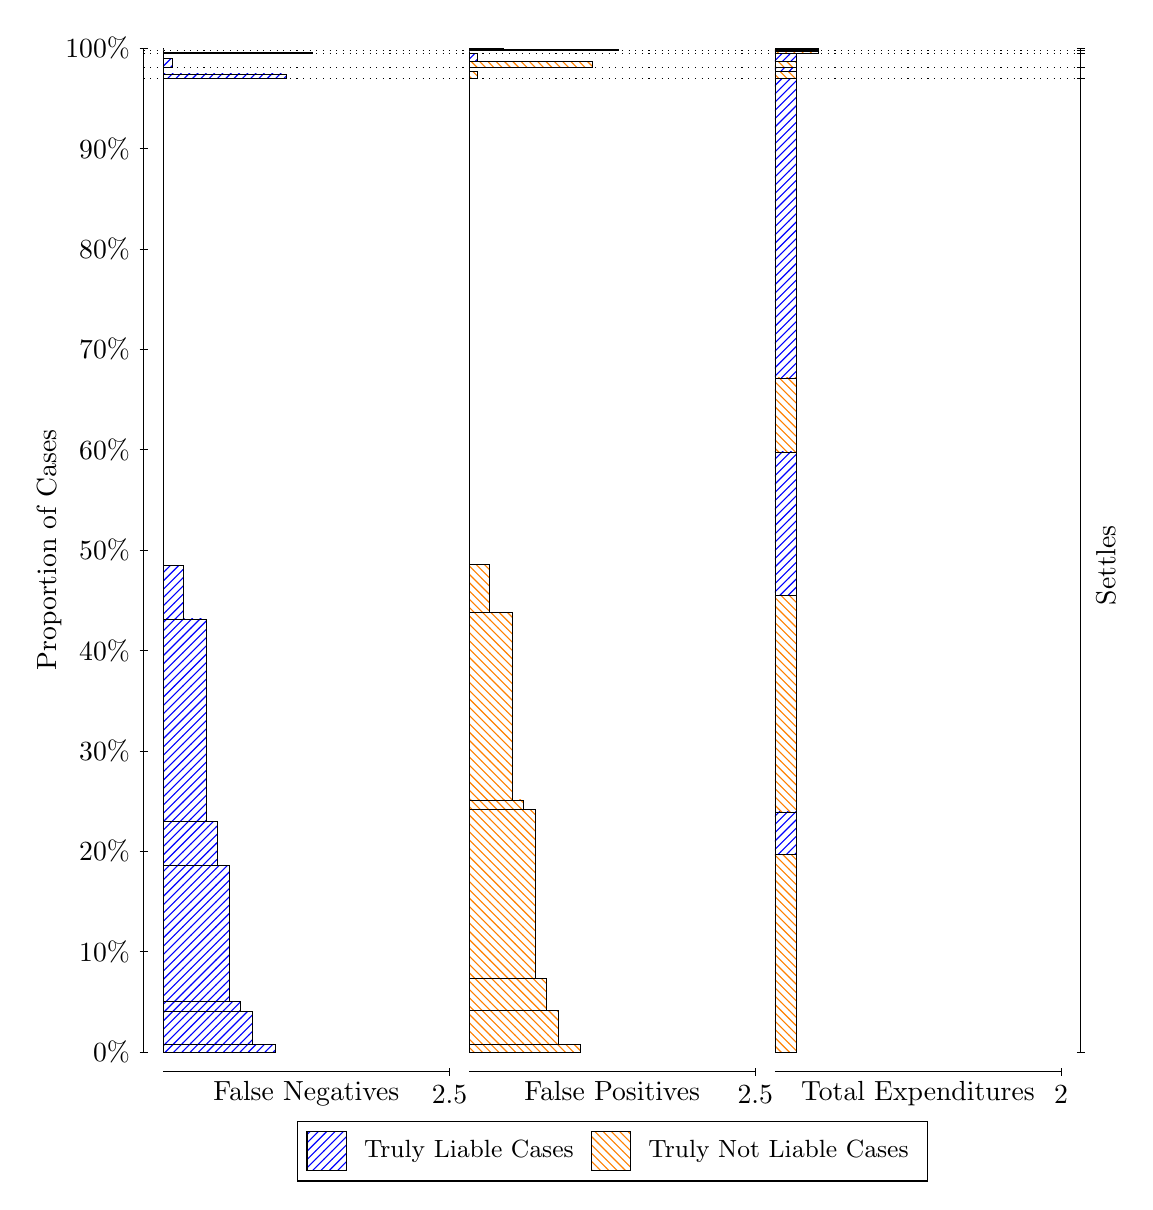
\begin{tikzpicture}
\draw[black, very thin] (1.5,1.75) -- (1.5,14.5);
\node[rotate=90, text=black, anchor=center] at (0.3, 8.125) {Proportion of Cases};
\draw[black, very thin] (1.45,1.75) -- (1.55,1.75);
\node[text=black, anchor=east] at (1.45, 1.75) {0\%};
\draw[black, very thin] (1.45,3.025) -- (1.55,3.025);
\node[text=black, anchor=east] at (1.45, 3.025) {10\%};
\draw[black, very thin] (1.45,4.3) -- (1.55,4.3);
\node[text=black, anchor=east] at (1.45, 4.3) {20\%};
\draw[black, very thin] (1.45,5.575) -- (1.55,5.575);
\node[text=black, anchor=east] at (1.45, 5.575) {30\%};
\draw[black, very thin] (1.45,6.85) -- (1.55,6.85);
\node[text=black, anchor=east] at (1.45, 6.85) {40\%};
\draw[black, very thin] (1.45,8.125) -- (1.55,8.125);
\node[text=black, anchor=east] at (1.45, 8.125) {50\%};
\draw[black, very thin] (1.45,9.4) -- (1.55,9.4);
\node[text=black, anchor=east] at (1.45, 9.4) {60\%};
\draw[black, very thin] (1.45,10.675) -- (1.55,10.675);
\node[text=black, anchor=east] at (1.45, 10.675) {70\%};
\draw[black, very thin] (1.45,11.95) -- (1.55,11.95);
\node[text=black, anchor=east] at (1.45, 11.95) {80\%};
\draw[black, very thin] (1.45,13.225) -- (1.55,13.225);
\node[text=black, anchor=east] at (1.45, 13.225) {90\%};
\draw[black, very thin] (1.45,14.5) -- (1.55,14.5);
\node[text=black, anchor=east] at (1.45, 14.5) {100\%};

\draw[black, very thin] (13.4,1.75) -- (13.4,14.5);
\draw[black, very thin] (13.35,1.75) -- (13.45,1.75);
\node[anchor=west] at (13.35, 1.75) {};
\draw[black, very thin] (13.35,14.115) -- (13.45,14.115);
\node[anchor=west] at (13.35, 14.115) {};
\draw[black, very thin] (13.35,14.258) -- (13.45,14.258);
\node[anchor=west] at (13.35, 14.258) {};
\draw[black, very thin] (13.35,14.435) -- (13.45,14.435);
\node[anchor=west] at (13.35, 14.435) {};
\draw[black, very thin] (13.35,14.468) -- (13.45,14.468);
\node[anchor=west] at (13.35, 14.468) {};
\draw[black, very thin] (13.35,14.5) -- (13.45,14.5);
\node[anchor=west] at (13.35, 14.5) {};

\draw[black, very thin, pattern color=blue, pattern=north east lines] (1.75,1.75) rectangle (3.167,1.8429);
\draw[black, very thin, pattern color=blue, pattern=north east lines] (1.75,1.8429) rectangle (2.8763,2.2655);
\draw[black, very thin, pattern color=blue, pattern=north east lines] (1.75,2.2655) rectangle (2.731,2.3882);
\draw[black, very thin, pattern color=blue, pattern=north east lines] (1.75,2.3882) rectangle (2.5857,4.1211);
\draw[black, very thin, pattern color=blue, pattern=north east lines] (1.75,4.1211) rectangle (2.4403,4.675);
\draw[black, very thin, pattern color=blue, pattern=north east lines] (1.75,4.675) rectangle (2.295,7.2509);
\draw[black, very thin, pattern color=blue, pattern=north east lines] (1.75,7.2509) rectangle (2.0043,7.9264);
\draw[black, very thin, pattern color=orange, pattern=north west lines] (1.75,7.9264) rectangle (1.75,14.115);
\draw[black, very thin, pattern color=blue, pattern=north east lines] (1.75,14.115) rectangle (3.3123,14.172);
\draw[black, very thin, pattern color=orange, pattern=north west lines] (1.75,14.172) rectangle (1.75,14.258);
\draw[black, very thin, pattern color=blue, pattern=north east lines] (1.75,14.258) rectangle (1.859,14.367);
\draw[black, very thin, pattern color=orange, pattern=north west lines] (1.75,14.367) rectangle (1.75,14.435);
\draw[black, very thin, pattern color=blue, pattern=north east lines] (1.75,14.435) rectangle (3.6393,14.446);
\draw[black, very thin, pattern color=orange, pattern=north west lines] (1.75,14.446) rectangle (1.75,14.468);
\draw[black, very thin, pattern color=orange, pattern=north west lines] (1.75,14.468) rectangle (1.75,14.479);
\draw[black, very thin, pattern color=blue, pattern=north east lines] (1.75,14.479) rectangle (1.75,14.5);
\draw[black, very thin, pattern color=orange, pattern=north west lines] (5.6333,1.75) rectangle (7.0503,1.8489);
\draw[black, very thin, pattern color=orange, pattern=north west lines] (5.6333,1.8489) rectangle (6.7597,2.2792);
\draw[black, very thin, pattern color=orange, pattern=north west lines] (5.6333,2.2792) rectangle (6.6143,2.6884);
\draw[black, very thin, pattern color=orange, pattern=north west lines] (5.6333,2.6884) rectangle (6.469,4.8282);
\draw[black, very thin, pattern color=orange, pattern=north west lines] (5.6333,4.8282) rectangle (6.3237,4.9509);
\draw[black, very thin, pattern color=orange, pattern=north west lines] (5.6333,4.9509) rectangle (6.1783,7.3332);
\draw[black, very thin, pattern color=orange, pattern=north west lines] (5.6333,7.3332) rectangle (5.8877,7.9386);
\draw[black, very thin, pattern color=blue, pattern=north east lines] (5.6333,7.9386) rectangle (5.6333,14.115);
\draw[black, very thin, pattern color=orange, pattern=north west lines] (5.6333,14.115) rectangle (5.7423,14.2);
\draw[black, very thin, pattern color=blue, pattern=north east lines] (5.6333,14.2) rectangle (5.6333,14.258);
\draw[black, very thin, pattern color=orange, pattern=north west lines] (5.6333,14.258) rectangle (7.1957,14.326);
\draw[black, very thin, pattern color=blue, pattern=north east lines] (5.6333,14.326) rectangle (5.7423,14.435);
\draw[black, very thin, pattern color=orange, pattern=north west lines] (5.6333,14.435) rectangle (5.6333,14.457);
\draw[black, very thin, pattern color=blue, pattern=north east lines] (5.6333,14.457) rectangle (5.6333,14.468);
\draw[black, very thin, pattern color=orange, pattern=north west lines] (5.6333,14.468) rectangle (7.5227,14.479);
\draw[black, very thin, pattern color=blue, pattern=north east lines] (5.6333,14.479) rectangle (6.0693,14.5);
\draw[black, very thin, pattern color=orange, pattern=north west lines] (9.5167,1.75) rectangle (9.7892,4.255);
\draw[black, very thin, pattern color=blue, pattern=north east lines] (9.5167,4.255) rectangle (9.7892,4.8003);
\draw[black, very thin, pattern color=orange, pattern=north west lines] (9.5167,4.8003) rectangle (9.7892,7.5454);
\draw[black, very thin, pattern color=blue, pattern=north east lines] (9.5167,7.5454) rectangle (9.7892,9.3712);
\draw[black, very thin, pattern color=orange, pattern=north west lines] (9.5167,9.3712) rectangle (9.7892,10.31);
\draw[black, very thin, pattern color=blue, pattern=north east lines] (9.5167,10.31) rectangle (9.7892,14.115);
\draw[black, very thin, pattern color=orange, pattern=north west lines] (9.5167,14.115) rectangle (9.7892,14.2);
\draw[black, very thin, pattern color=blue, pattern=north east lines] (9.5167,14.2) rectangle (9.7892,14.258);
\draw[black, very thin, pattern color=orange, pattern=north west lines] (9.5167,14.258) rectangle (9.7892,14.326);
\draw[black, very thin, pattern color=blue, pattern=north east lines] (9.5167,14.326) rectangle (9.7892,14.435);
\draw[black, very thin, pattern color=orange, pattern=north west lines] (9.5167,14.435) rectangle (10.062,14.457);
\draw[black, very thin, pattern color=blue, pattern=north east lines] (9.5167,14.457) rectangle (10.062,14.468);
\draw[black, very thin, pattern color=orange, pattern=north west lines] (9.5167,14.468) rectangle (10.062,14.479);
\draw[black, very thin, pattern color=blue, pattern=north east lines] (9.5167,14.479) rectangle (10.062,14.5);
\draw[black, dotted] (1.5,14.115) -- (13.4,14.115);
\draw[black, dotted] (1.5,14.258) -- (13.4,14.258);
\draw[black, dotted] (1.5,14.435) -- (13.4,14.435);
\draw[black, dotted] (1.5,14.468) -- (13.4,14.468);
\draw[black, very thin] (1.75,1.5) -- (5.3833,1.5);
\node[text=black, anchor=north] at (3.5667, 1.5) {False Negatives};
\draw[black, very thin] (5.3833,1.45) -- (5.3833,1.55);
\node[text=black, anchor=north] at (5.3833, 1.45) {2.5};

\draw[black, very thin] (5.6333,1.5) -- (9.2667,1.5);
\node[text=black, anchor=north] at (7.45, 1.5) {False Positives};
\draw[black, very thin] (9.2667,1.45) -- (9.2667,1.55);
\node[text=black, anchor=north] at (9.2667, 1.45) {2.5};

\draw[black, very thin] (9.5167,1.5) -- (13.15,1.5);
\node[text=black, anchor=north] at (11.333, 1.5) {Total Expenditures};
\draw[black, very thin] (13.15,1.45) -- (13.15,1.55);
\node[text=black, anchor=north] at (13.15, 1.45) {2};

\node[text=black, centered, rotate=90] at (13.72, 7.9325) {Settles};





\draw (7.449999999999999,1.5) node[draw=none] (baseCoordinate) {};
\begin{scope}[align=center]
        \matrix[scale=0.5, draw=black, below=0.5cm of baseCoordinate, nodes={draw}, column sep=0.1cm]{
            \node[rectangle, draw, minimum width=0.5cm, minimum height=0.5cm, pattern color=blue, pattern=north east lines] {}; &
            \node[draw=none, font=\small, text=black] (B) {Truly Liable Cases}; &
            \node[rectangle, draw, minimum width=0.5cm, minimum height=0.5cm, pattern color=orange, pattern=north west lines] {}; &
            \node[draw=none, font=\small, text=black] (B) {Truly Not Liable Cases}; \\
            };
\end{scope}

\end{tikzpicture}
\end{document}